% \documentclass[preprint]{kcc}
\documentclass{kcc}


%%%%%%%%%%%%%%%%%%%%%%%%%%%%%%%%%%%%%%%%%%%%%%%
% include additional packages you need to use
%%%%%%%%%%%%%%%%%%%%%%%%%%%%%%%%%%%%%%%%%%%%%%%
% graphic, float package
\usepackage{graphicx}		% for setting images
\usepackage{float}			% for float objects
\usepackage{subfigure}	% for adding several figures in a figure environment
\usepackage{lscape}			% for landscape type images or tables

% Reduce the line spacing in the bibliography
\let\oldbibliography\thebibliography
\renewcommand{\thebibliography}[1]{%
  \oldbibliography{#1}%
  \setlength{\itemsep}{0pt}%
}

\usepackage{enumitem}

% for compact section title spacing
% \usepackage[compact]{titlesec}

% nameref
\usepackage{nameref}

% mathmetical presentation
\usepackage{gensymb}
\usepackage{amsmath}
\usepackage{amssymb}
\usepackage{amsthm}
\usepackage{exscale}
\usepackage{textcomp}		% extra symbols


% for circled number
\newcommand{\cl}[1]{\textcircled{\scriptsize #1}}


% package for using algorithmic presentation
\usepackage{algorithmic}
\usepackage{algorithm}
% customize algorithmic environment
\renewcommand{\algorithmicrequire}{\makebox[40px]{\hfill\textbf{Input :}}}
\renewcommand{\algorithmicensure}{\makebox[40px]{\hfill\textbf{Output :}}}

% array and table presentation
\usepackage{array}
\usepackage{tabulary}
\usepackage{multirow}
\usepackage[table]{xcolor}
\usepackage{ctable}
\usepackage{booktabs}		% for typesetting tables at the level of publication		
							% do not use vertical rule
							
% set title, author, abstract
\title{비디오 시청 환경에서의 장기 기억에 대한 안구 운동 분석}
\author{
김진화$^{\circ1}$, 장병탁$^{12}$\\
서울대학교 인지과학 협동과정$^{1}$\\
서울대학교 컴퓨터공학부$^{2}$\\
\{jhkim, btzhang\}@bi.snu.ac.kr
}
\engtitle{Eye Movement Analysis for Long-term Memory on Video Stimuli}
\engauthor{
Jin-Hwa Kim$^{\circ1}$, Byoung-Tak Zhang$^{1234}$\\
Cognitive Science Program$^{1}$, School of Computer Science and Engineering$^{2}$, Seoul National University\\
}
\abstract{
안구 운동은 뇌 활동을 관찰할 수 있는 비침습적이면서 활용도가 높은 지표이다. 이러한 배경으로 최근 안경류 웨어러블 장비가 연구 기관을 중심으로 빠르게 보급되고 있으며 안구 운동에 대한 연구 활동과 관련 산업의 성장을 고도화 하고 있다. 우리는 아동용 비디오 시청 환경에서 안구 운동을 연구하였다. 응시 기간에 따른 장기 기억 상관 여부를 확인해 보았지만 유의성을 발견할 수 없었다. 하지만 시청 자극을 주의 상황과 중립 상황으로 나눈 후 응시 기간에 따른 차이를 확인하였을 때 긴 응시에서는 장기 기억 인출에서 통계적으로 유의미한 차이를 발견할 수 있었지만 짧은 응시에서는 그렇지 못하였다. 이러한 안구 운동의 특징에서 발견되는 장기 기억과 관련된 인지 처리 과정은 평생 학습 기제에서 선택적 주의를 통한 효율성 추구가 제한된 인지 처리 능력 안에서 중요한 요소로 기여함을 시사한다.
}


\begin{document}

\maketitle


\section{서 론}
\iffalse
안구 운동은 물리적으로 여섯 개의 근육을 이용하여 시선을 움직이고 고정시킨다. 이 여섯 개의 근육은 상하 좌우 및 회전하는 방향으로 각각 두 개의 근육이 수축하고 이완하며 조절한다. 이러한 근육 운동은 자율적으로 또는 무의식적으로 일어나는데 뇌로부터 안구 운동에 이르는 신경 신호 전달 경로는 하나 이상으로 다양한 영역에서 관여한다.
\fi

안구 운동 측정기로부터 관찰되는 안구 운동은 크게 세가지로 분류할 수 있다. 첫번째는 한 지점을 바라보는 고정 상태인 응시이다. 응시는 의도적으로 주의를 기울여도 완벽히 한 지점을 바라볼 수 없는데 안구 근육의 수축 또는 이완의 상태를 유지하는 데 분자 수준에서의 지속적인 화학 반응이 필요하기 때문이다. 두번째는 도약 운동이다. 응시와 응시 사이에는 상대적으로 빠른 안구 움직임이 있는데 이를 도약 운동이라고 한다. 응시와 도약 운동을 분리하는 일은 실험의 목적에 따라 특별히 고안된 여과 함수를 통해 수행한다. 가장 많이 사용하는 여과 방법으로는 초당 움직인 각도를 기준으로 응시와 도약 운동을 분류하며 일반적으로 초당 30 도 이상 움직이게 되면 도약 운동으로 분류한다. 세번째는 부드러운 추적 운동이다. 천천히 움직이는 시각 자극을 쫓는 시선 궤적은 초당 30 도 이하의 속력으로 움직이지만 경향성을 가진 시선 이동을 만들어 낸다. 본 논문에서는 부드러운 추적 운동에 대한 분석은 생략하였다.

많은 심리학자들과 신경과학자들에 의해 읽기 환경에서 안구 운동을 연구 하였다 \cite{Rayner1998,Reichle1998}. 특히 통제된 읽기 자료를 이용한 안구 운동 연구\cite{Inhoff1986,Rayner1986}는 단어 빈도 수 등과 같은 언어학적 특징과 응시 기간의 관련성을 보이며 응시 기간을 인지 처리 작업량을 나타내는 지표로 해석하기 시작했다. 

시청 환경에서는 감정을 유발하는 장면이나 내용의 문맥이 긴 응시를 유발할 수 있다. 다음 응시를 선택하거나 도약 운동 방향을 결정할 때는, 단어 배치 분포를 따라 좌우 이동이 우세한 읽기 환경과는 달리 훨씬 자유롭다는 점에서 중요한 차이를 보인다.

따라서 시청 환경에서의 안구 운동 분석은 읽기 환경과 비교할 때 연구의 복잡성 증가\cite{Choe2013}와 방법론적 어려움 때문에 충분히 연구되지 못하고 있었다 \cite{Tatler2011}. 하지만 최근에는 구글 글래스와 같은 웨어러블 장비의 개발과 휴대용 안구 운동 측정기의 보급은 보다 자유로운 환경에서의 실험을 가능하게 했고 안구 운동 연구 주제 범위를 넓혔으며 시각 자극의 현저점 분석 기법\cite{itti1998model}은 다양한 응용 기술 개발을 촉진시켰다. 

본 논문에서는 시청 환경에서 안구 운동을 장기 기억 형성과 관련하여 분석하였다. 안구 운동을 응시와 도약 운동으로 분류한 후 \cite{Findlay1999,Feng2003,Feng2006}, 응시 기간과 장기 기억 형성이 서로 상관 관계가 있는지 분석하여 시청 환경에서도 응시 기간이 장기 기억와 관련된 인지 처리의 지표로 볼 수 있는지 확인하였다. 또한 감정적 유발 영상이 장기 기억 형성과 관련되어 있다는 선행 연구 \cite{Cahill1996amyg,Cahill1998baso}를 바탕으로 응시 기간이 감정적 유발 영상에 대한 장기 기억 형성을 나타내는 지표가 될 수 있는 지 확인하였다. 

\section{실험 설계}

\subsection{실험 1}
본 연구를 위하여 세계적으로 유명한 아동용 애니메이션인 뽀로로 시즌 3의 에피소드 1-13을 사용하였다. 

우리는 18명의 뽀로로 시즌 3을 처음으로 보는 참여자 (남자 11명, 여자 6명; 나이 중간 값 25 세)를 모집하였다. 본 연구의 실험은 서울대학교 생명윤리심의 위원회의 동의를 얻어 진행하였고 모든 참여자는 연구 참여 동의서를 작성한 후 실험에 참여하였다.

참여자는 차광막으로 둘러쌓인 약 3 평의 공간에서 40 인치 와이드 스크린 HDTV를 시선 거리 1.7 m 앞의 쇼파에 앉아 시청하였다. 안구 운동과 참여자 시야는 \textit{Tobii Glasses} 안구 운동 측정기의 적외선 카메라와 일반 카메라를 이용하여 각각 녹화 (30 Hz) 하였다. 안구 운동 중 응시를 구분하기 위해 초당 30 도 미만의 이동을 응시로 구분하는 \textit{I-VT} 알고리즘을 사용하였다. 안구 운동의 일반적인 움직임은 초당 100 도 이하의 낮은 속도와 초당 300도 이상의 높은 속도로 구분할 수 있기 때문에 속도 기반 분류는 간단하지만 높은 성능을 보인다 \cite{Salvucci2000}. 우리는 이렇게 측정된 안구 운동을 응시와 도약 운동 두 종류로 분류하였는데 측정 오류로 인한 분류가 되지 않는 값은 사용되지 않았다. 


\subsection{실험 2}
\label{subsec:experiment2}
실험 1을 참여했던 11명의 참여자를 대상으로 실험 1의 안구 운동 측정 데이터를 바탕으로 각 참여자를 위해 준비한 기억 능력 시험을 준비하였다. 실험 2는 실험 1을 실시한 지 3 개월에서 4 개월 사이의 기간 후 실시 하였다 (실험 일정 조정으로 인해 수 일의 차이가 존재 하였다.).

기억 능력 시험은 총 20 개의 3 초 가량의 짧은 동영상으로 구성되어 있다. 8개의 동영상은 300 ms 미만의 응시 기간을 가지는 \textit{짧은 응시} 동영상이고, 다른 8개의 동영상은 1400 ms 이상의 응시 기간을 가지는 \textit{긴 응시} 동영상이다. 나머지 4개의 동영상은 같은 뽀로로 시리즈의 다른 시즌 영상에서 추출한 짧은 동영상으로 참여자가 실험 1에서 보지 않았던 내용이다.

각 참여자는 20 개의 짧은 동영상이 무작위로 정렬된 기억 능력 시험을 응하게 된다. 각 동영상은 실험 1에서 본 동영상인지 아닌지 1 점에서 5 점의 확신 정도를 점수로 매기게 된다. 


\section{결 과}
그림~\ref{fig:memtest-leng}는 긴 응시와 짧은 응시에 대한 기억 능력 테스트 결과를 나타낸다. 긴 응시와 짧은 응시에 대한 자세한 설명은 ~\nameref{subsec:experiment2} 소절을 참조한다. 긴 응시와 짧은 응시에 대한 기억력 점수는 통계적으로 유의미 하지 않았는데 시청 환경에서의 긴 응시에는 인지적 처리 외에도 다른 요인이 있다는 것을 나타낸다. 이를 분석하기 위해 시각 자극의 종류를 고려하였다.

감정적 유발 영상이 장기 기억 형성과 관련되어 있다는 선행 연구 \cite{Cahill1996amyg,Cahill1998baso}를 바탕으로 응시 기간이 감정적 유발 영상에 대한 장기 기억 형성을 나타내는 지표가 될 수 있는 지에 대해 분석하였다. 그림~\ref{fig:memtest-nested}는 그 분석 결과를 나타낸다. 긴 응시에서는 선행 연구에서와 같이 감정적 유발 영상에 대한 효과가 통계적으로 유의미하게 나타나지만 짧은 응시에서는 그렇지 못했다. 자세한 내용은 그림~\ref{fig:memtest-nested}의 설명문을 참조한다.

\begin{figure}
  \centerline{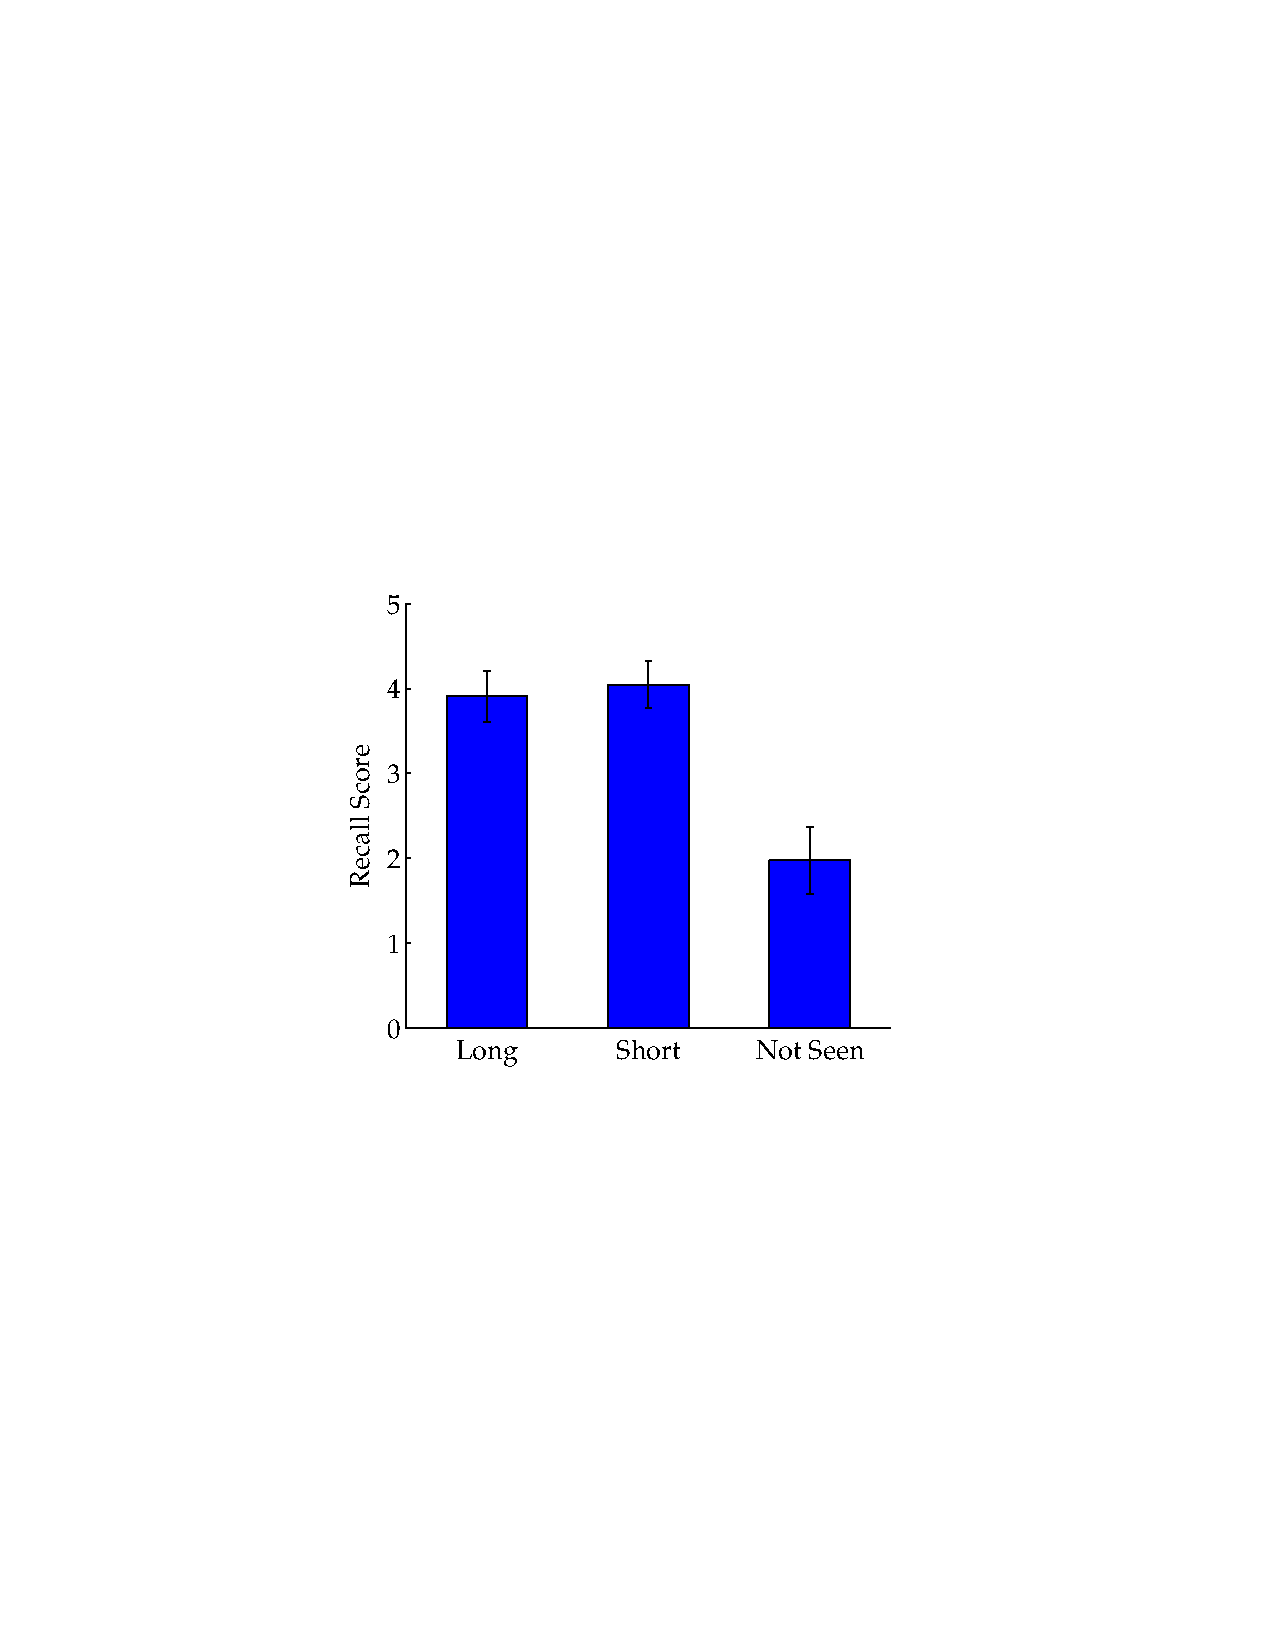
\includegraphics[width=60mm,height=54mm,trim=65mm 103mm 68mm 100mm]{./eps/memtest_leng}}
  \caption{긴 응시와 짧은 응시에 대한 장기 기억 능력 시험 결과 이다. 긴 응시와 짧은 응시에 대한 기억력 점수는 통계적으로 유의미 하지 않았다 (p $=$ 0.5051). 오차 막대는 $\pm$ 2 표준 오차를 뜻 한다. 실험에 대한 자세한 설명은 ~\nameref{subsec:experiment2} 소절을 참조한다.}
  \label{fig:memtest-leng}
\end{figure}

\begin{figure}
  \centerline{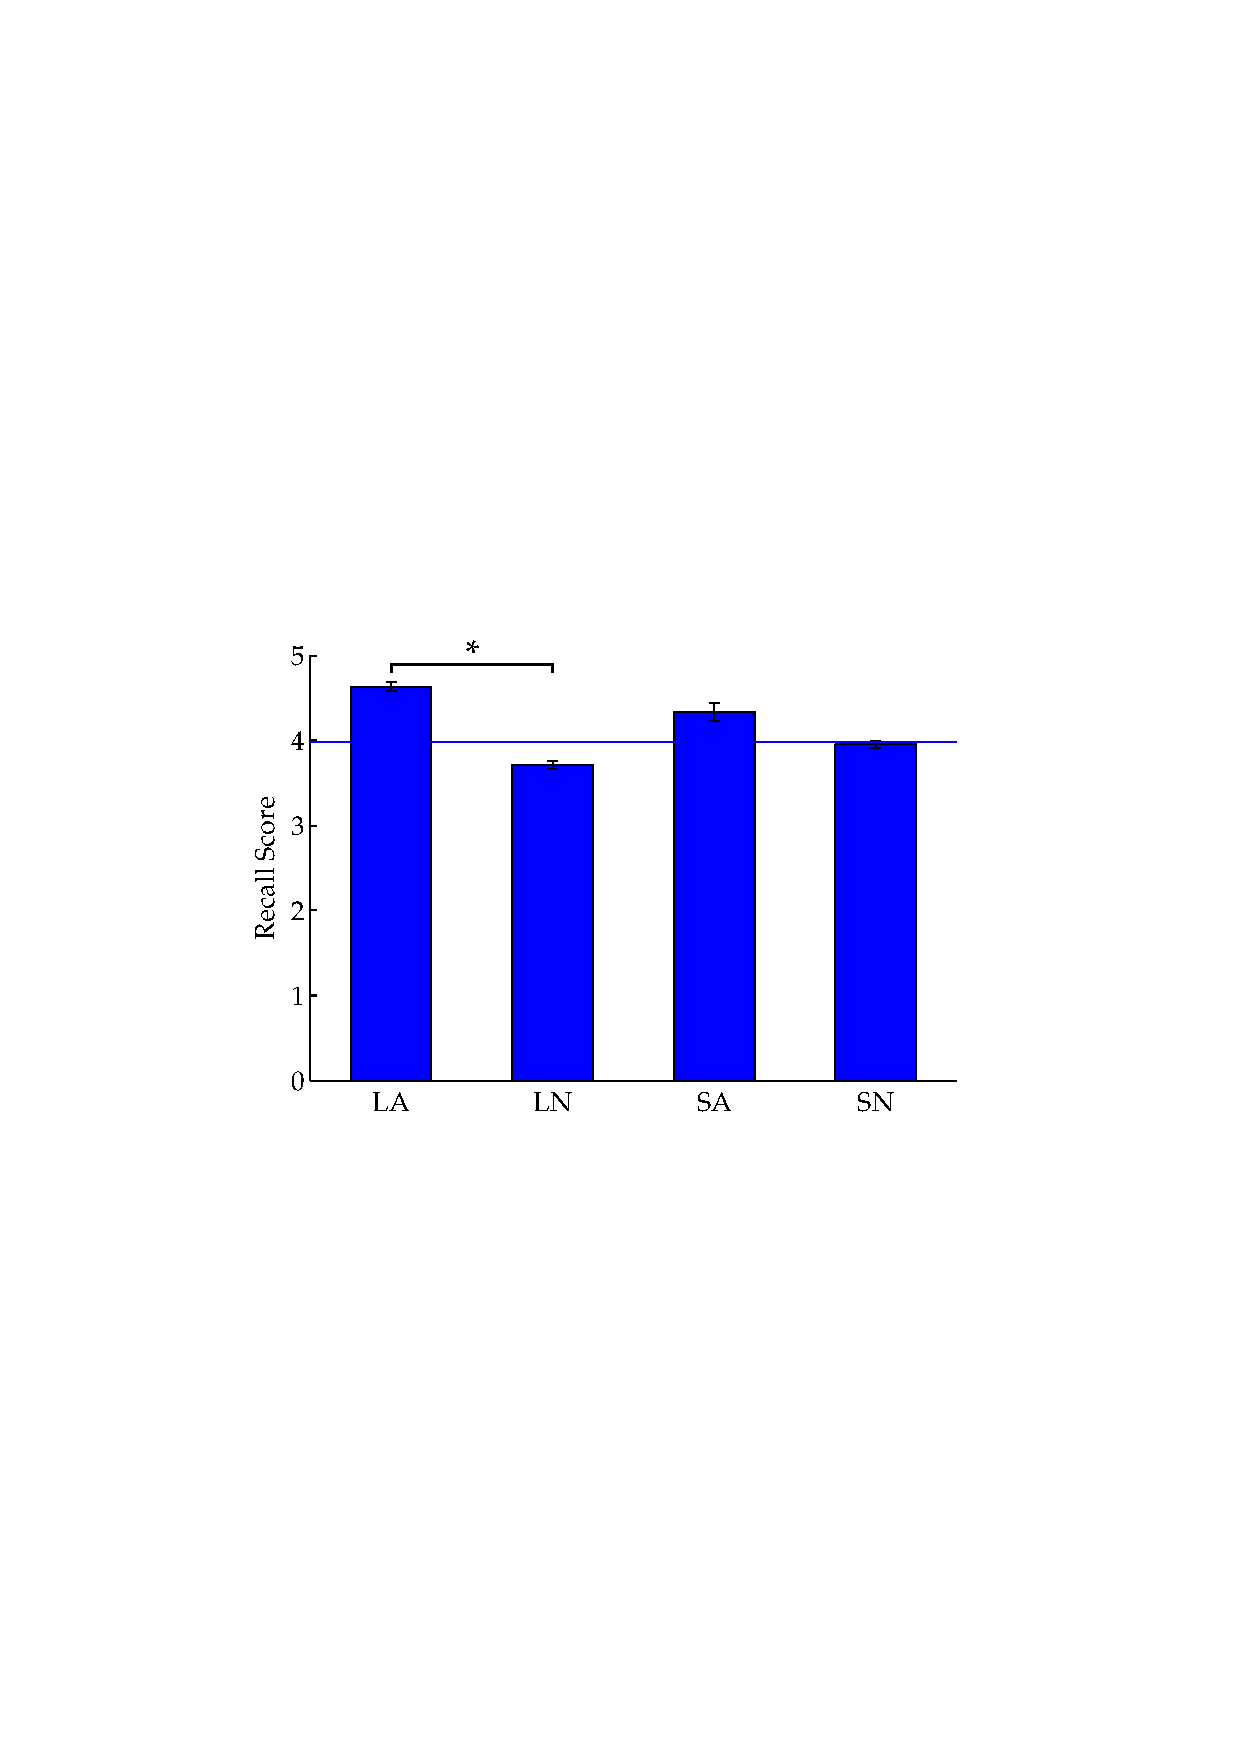
\includegraphics[width=60mm,height=54mm,trim=55mm 108mm 58mm 105mm]{./eps/memtest_nested}}
  \caption{응시 길이에 따른 감정적 유발을 일으키는 감정 자극의 장기 기억 형성 영향도를 분석하였다. 실험 2에서 11 명의 참여자에게 채점을 받은 긴 응시 동영상은 총 88 개로, 감정 자극이 포함된 동영상은 19개, 중립 동영상은 69개 이다. 두 평균의 차이는 통계적으로 유의미 하였다 (p = 0.0104 $<$ 0.05). 짧은 응시 동영상은 긴 응시 동영상과 같이 총 88 개로, 감정 자극이 포함된 동영상은 21개, 중립 동영상은 67개 이다. 이 두 평균 의 차이는 통계적으로 유의미 하지 않았다. 파란 가로 줄은 모든 동영상의 평균 점수를 나타낸다. 오차 막대는 $\pm$ 2 표준 오차를 나타낸다. LA는 감정 자극에 대한 긴 응시, LN은 중립 자극에 대한 긴 응시, SA는 감정 자극에 대한 짧은 응시, SN은 중립 자극에 대한 짧은 응시를 나타낸다.}
  \label{fig:memtest-nested}
\end{figure}


\section{토 론}
응시 기간에 따른 분석에서 기억 점수의 차이를 확인할 수 없었지만 응시 기간에 따른 감정 자극 효과를 관찰함으로써 장기 응시는 주의와 관련 있음을 확인할 수 있었다. 선행 연구 \cite{Cahill1996amyg,Cahill1998baso}에서 나타나는 감정 효과가 짧은 응시에서는 분명히 나타나지 않지만 상대적으로 장기 응시에서 확인할 수 있기 때문이다. 시청 환경에서 장기 응시는 읽기 환경에서와 같이 감정 자극을 이해하도록 인지 처리를 수행하고 있는 지표로 제한적으로 볼 수 있다 \cite{Rayner1997}. 

하지만 중립 자극에 대한 장기 응시는 기억 점수에서 가장 낮은 값을 가졌는데, 몇 가지의 해석 가능성이 있다. 시각 자극의 규칙적 특성으로 인해 시선 이동을 제한한 것, 예를 들면, 반복적으로 화면 가운데 나타나는 캐릭터, 화면에서 시각 자극의 변경이 거의 없는 경우가 있다. 이것은 시각 자극에서 주의 요소가 없거나 주의가 떨어진 상태에서 적극적으로 시각 자극 탐색을 하지 않았다고도 할 수 있다. 본문에서는 생략하였지만 주의 자극은 중립 자극에 비하여 장기 응시로 분류된 안구 운동의 시선 위치에 대한 분산 값이 유의미하게 낮았다. 



\section{결 론}
우리는 본문을 통해 아동용 비디오 시청 환경에서 장기 기억과 관련이 있는 안구 운동 특징을 연구하였다. 응시 기간에 따른 장기 기억 정도는 직접적인 관련성을 발견할 수 없었지만 응시 기간에 따른 주의 상황과 중립 상황애서의 기억 정도의 차이를 확인하였을 때 긴 응시에서는 통계적으로 유의미한 차이를 발견할 수 있었고, 짧은 응시에서는 그렇지 못하였다. 이는 평생 학습에서 선택적 주의를 통한 효율성 추구가 제한된 인지 처리 능력을 극복할 수 있는 요소가 될 수 있음을 알려준다.


\section{감사의 글}
이 논문은 정부(미래창조과학부)의 재원으로 한국연구재단의 지원을 받아 수행된 연구이며(NRF-2010-0017734-Videome),
정부(미래창조과학부 및 정보통신기술진흥센터)의 정보통신·방송 연구개발사업 지원 (10035348-mLife, 14-824-09-014, 10044009-HRI.MESSI)을 일부 받았음.

\bibliographystyle{ieeetr}
\bibliography{../Thesis/kim2014activelong}

\end{document}
